\documentclass{article}

\usepackage[margin=1in]{geometry}
\usepackage[utf8]{inputenc}
\usepackage[english]{babel}
\usepackage{amsthm} %lets us use \begin{proof}
\usepackage{amssymb} %gives us the character \varnothing
\usepackage{xcolor}
\usepackage{float}
\usepackage{braket}
\usepackage{multirow}
\usepackage{array}
\usepackage{mathtools}
\usepackage{diagbox}
\usepackage{gensymb}

\title{Chem231B: Hw 4} % Title of the assignment

\begin{document}

\maketitle

\section*{\textbf{BO Approx}}

a) Making the BO approximation, write the purely electronic Hamiltonian and, by
completing the square, write its energy levels $E_{\text{el,n}}(X)$.

{\color{blue}
The full Hamiltonian ($\hat{H}$), the full wavefunction ($\Psi(x,X)$),
and the Schr\"odinger equation are defined,
\begin{align}
  \hat{H}\Psi(x,X) & = E_{\text{tot}}\Psi(x,X) \\
  \Psi(x,X) & = \phi_{\text{el}}(x)\phi_{\text{nuc}}(X) \\
  \hat{H} & = \hat{T}_{\text{nuc}} + \hat{T}_{\text{el}} + V(X,x).
\end{align}

Given: $V(X,x) = \frac{1}{2}(X^2+x^2) + \frac{1}{2}(x-X)^2$

Rearrange $V(X,x)$ and completing the square,
\begin{align}
  V(X,x) & = \frac{1}{2}(X^2+x^2) + \frac{1}{2}(x-X)^2 \nonumber \\
  & = \frac{1}{2}X^2+\frac{1}{2}x^2 + \frac{1}{2}(x^2-2xX+X^2) \nonumber \\
  & = X^2 + x^2 - xX
\end{align}

Perform coordinate transformation by substituting in $y=x-X/2$.
Hence, the purely electronic Hamiltonian is,
\begin{align}
  V(X,y) & = y^2 + xX - xX - \frac{X^2}{4} + X^2 \nonumber\\
  & = y^2 + \frac{3X^2}{4} \\
  \hat{H}_{\text{el}} & = \hat{T}_{\text{el}} + V(X,y) \nonumber\\
  & = \frac{p_y^2}{2} + y^2 +\frac{3X^2}{4}, \label{eqn:omega}
\end{align}

where $p_y$ is electronic momentum operator. The Sch\"odinger equation
for the electronic part,
\begin{align}
  \hat{H}_{\text{el}}\phi_{\text{el}}(x) & = E_{\text{el,n}}\phi_{\text{el}}(x) \\
  \Big(\frac{p_y^2}{2} + y^2 -\frac{3X^2}{4}\Big)\phi_{\text{el}}(x)
  & =E_{\text{el,n}}(X)\phi_{\text{el}}(x). \label{eqn:elec} \\
  E_{\text{el,n}}(X) & = \Big(n + \frac{1}{2}\Big)\omega_{\text{el}}
  + \frac{3X^2}{4}
\end{align}

$\omega_{el}$ is determined to be $\sqrt{2}$.}
\\

\noindent b) Write the nuclear equation for the proton in the field of the
electronic energy plus any other parts of the potential, to get an expression
for the totla energy of the system, $E_{\nu,n}$, where $\nu$ is the quantum
number for proton vibrations.
\\

{\color{blue}
Since the electronic part of the wavefunction is solved in part a), the
nuclear part is left,
\begin{align}
  (\hat{T}_{\text{nuc}} + E_{\text{el,n}}(X))\phi_{\text{nuc}}(X)
  & = E_{\text{tot}}\phi_{\text{nuc}}(X) \label{eqn:nuc} \\
  \Big(\frac{p_{\text{nuc}}}{2m_p} + \Big(n + \frac{1}{2}\Big)\omega_{\text{el}}
  + \frac{3X^2}{4}\Big)\phi_{\text{nuc}}(X) & = E_{\text{tot}}\phi_{\text{nuc}}(X)
\end{align}

Since the solutions are the harmonic oscillator, the total energy
($E_{\nu,n}$) is,
\begin{align}
  E_{\nu,n}& =\Big(\nu + \frac{1}{2}\Big)\omega_{\text{nuc}}
  + \Bigg(n+\frac{1}{2}\Bigg)\sqrt{2} \nonumber \\
  & = \Big(\nu + \frac{1}{2}\Big)\sqrt{\frac{3}{2m_p}}
  + \Bigg(n+\frac{1}{2}\Bigg)\sqrt{2}
\end{align}
where substituting $\omega_{\text{nuc}}=\sqrt{\frac{3}{2m_p}}.$
}

\noindent c) Assume $m=25$, plot the lowest 12 levels, labeling them with their
electronic and nuclear quantum numbers.

\begin{table}[H]
  \centering
  \caption{BO total energy in Hartree ($E_{\nu,n}$) for $m=25$, nuclear, and electronic
    quantum numbers $(\nu,n)$.}
  \begin{tabular}{c|cc}
    \diagbox{$\nu$}{$n$} & 0 & 1\\
    \hline
    0 & 0.830 & 2.244 \\
    1 & 1.075 & 2.489 \\
    2 & 1.319 & 2.734 \\
    3 & 1.564 & 2.979 \\
    4 & 1.809 & 3.224 \\
    5 & 2.054 & 3.469 \\
    6 & 2.299 & 3.713 \\
  \end{tabular}
\end{table}

\begin{figure}[H]
  \centering
  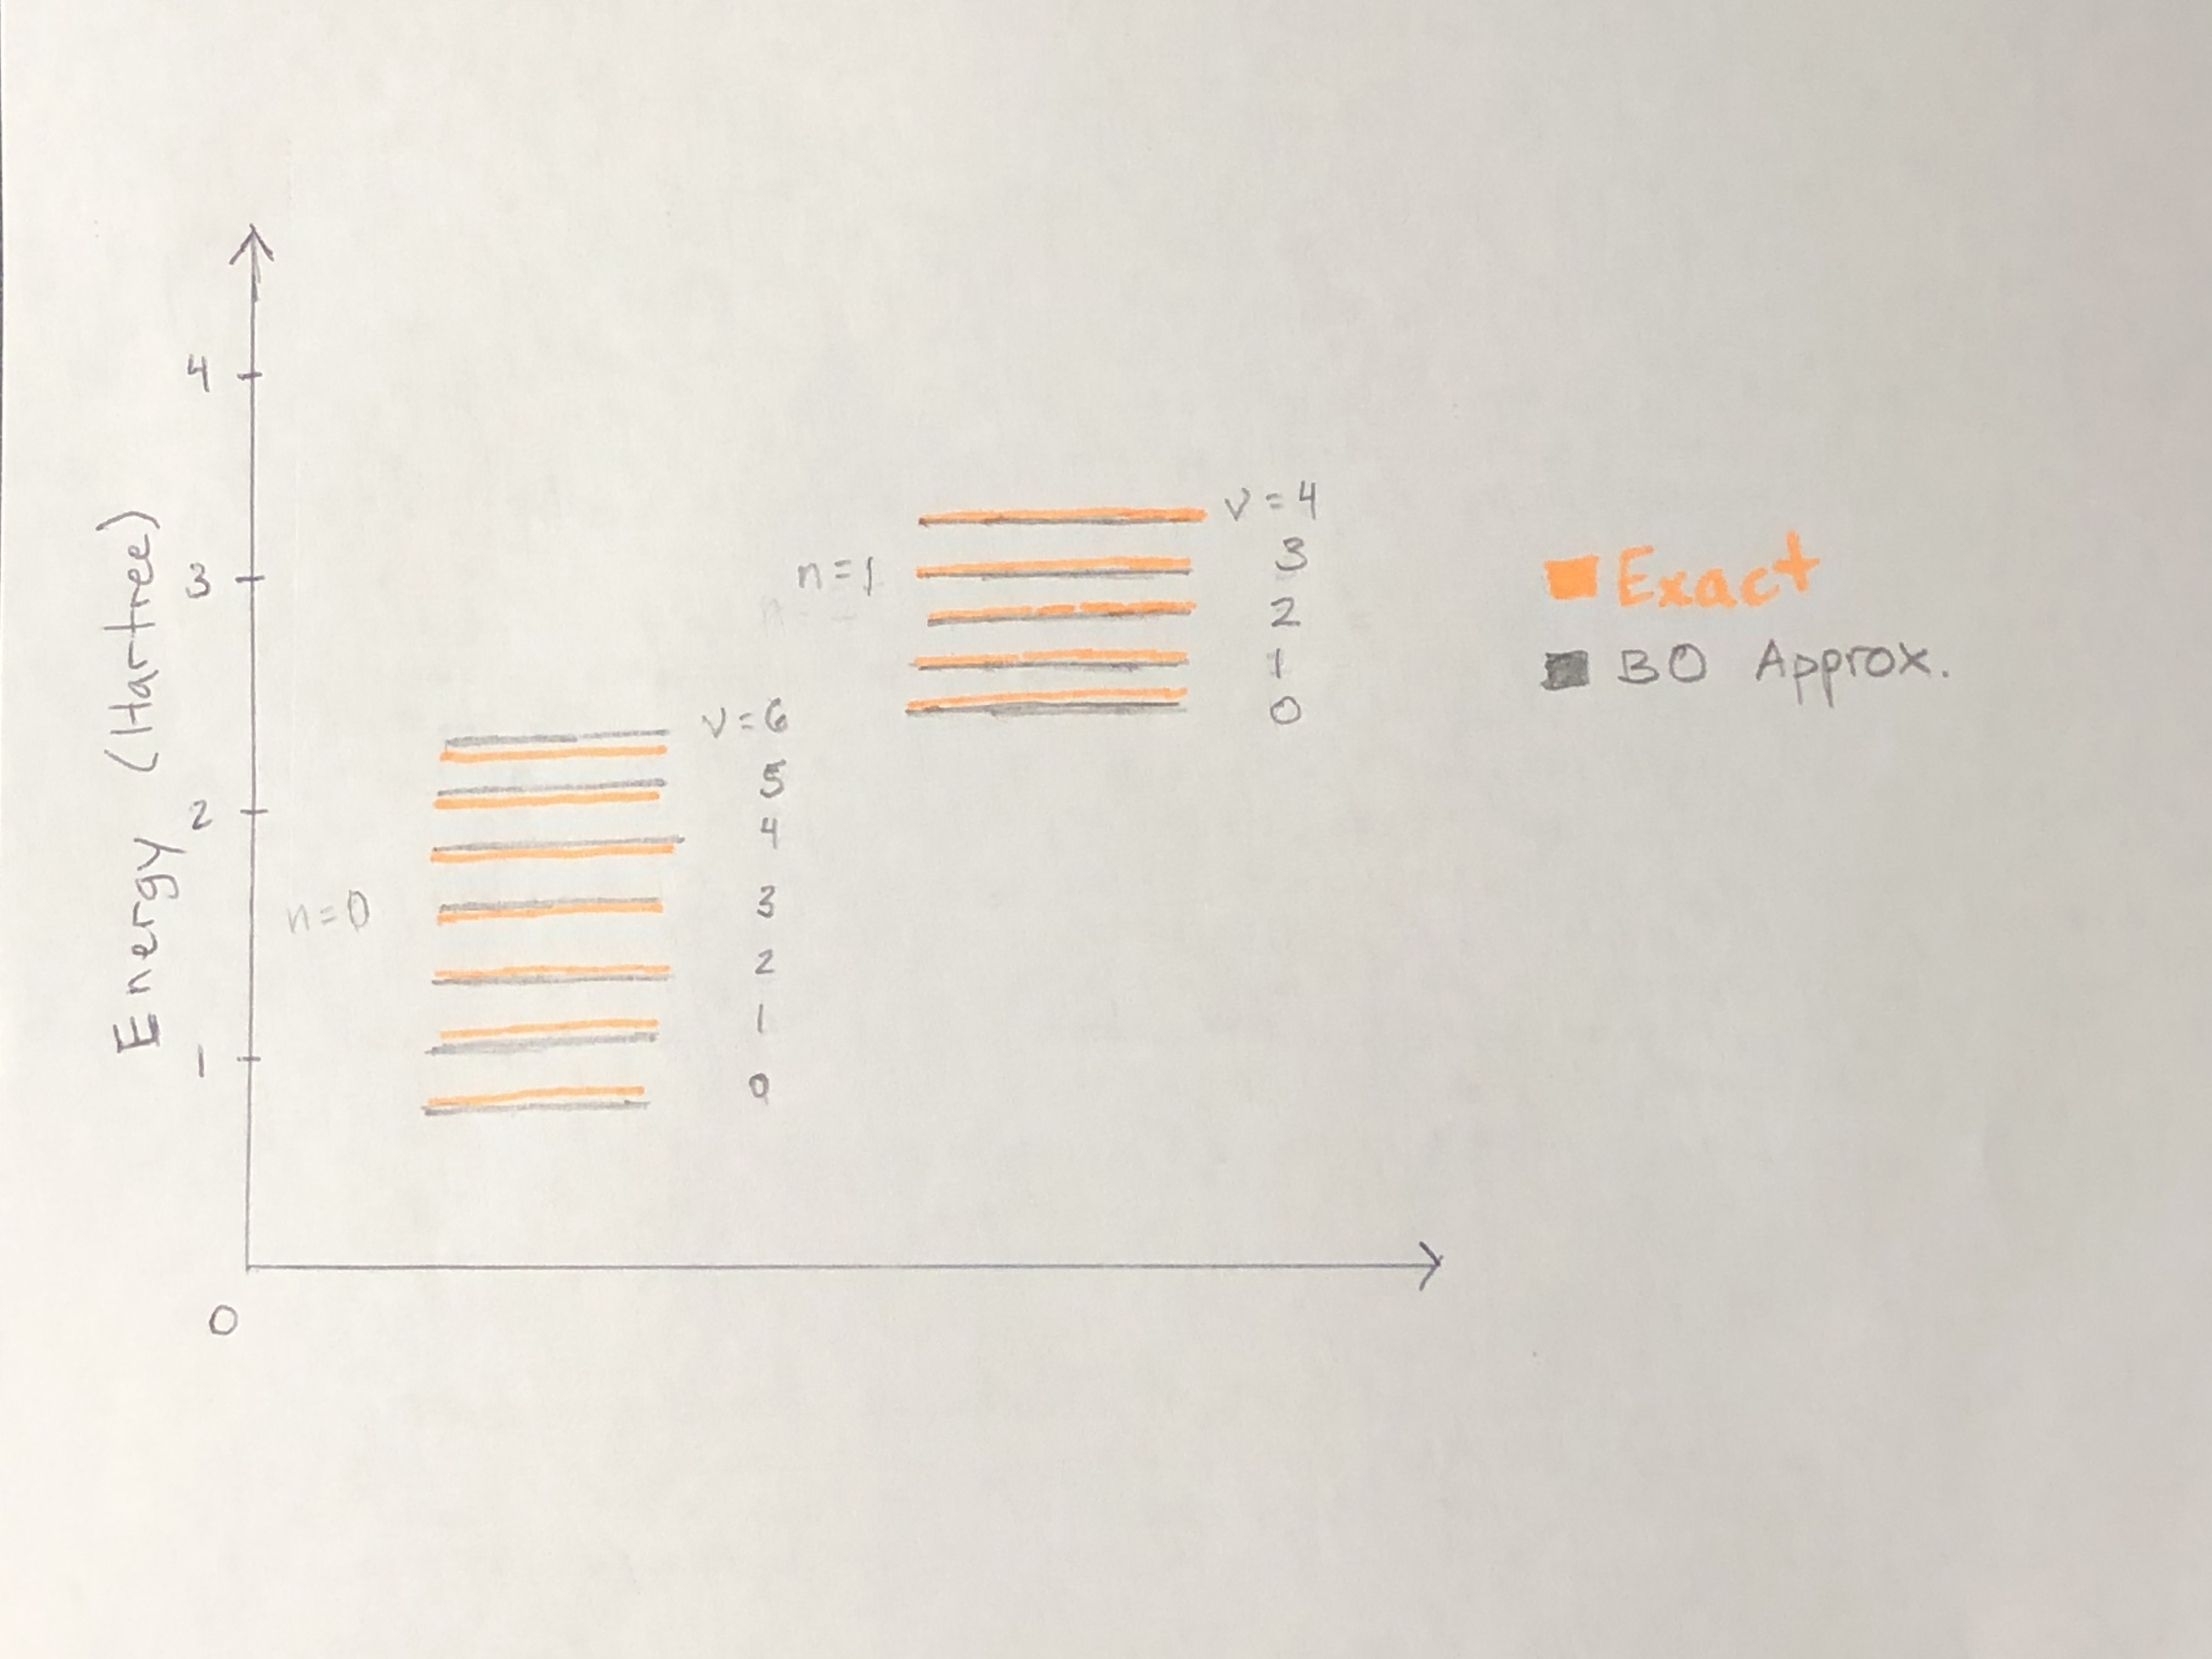
\includegraphics[scale=0.09]{bo_exact_energy.jpg}
  \caption{Energy spectrum of the exact and BO approximation energies
    for the electronic states ($n$) and vibrational states ($\nu$). The mass
    of proton is $m=25$.}
  \label{fig:bo}
\end{figure}

\noindent d) The exact solution to this problem is given by the sum of two harmonic
oscillators, with frequencies
\begin{equation}
  \omega_{\pm}^2 = 1 + \frac{1}{m}\pm\sqrt{1 - \frac{1}{m} + \frac{1}{m^2}}
  \label{eqn:omega}
\end{equation}
Show that, if $m >> 1$, this agree with your BO solutions above.
\\

{\color{blue}
  Rewrite Eqn \eqref{eqn:omega}

  \begin{equation}
    1 + \frac{1}{m}\pm(1-\frac{1}{2m})\sqrt{1+\frac{3}{4(m-1/2)^2}}
  \end{equation}
  
Exact solution is $E_{n',n}=\omega_+\Big(n+\frac{1}{2}\Big) + \omega_-\Big(n'+\frac{1}{2}\Big)$
and since $m>>1$, $\omega_+$ is determined to be
\begin{align*}
%  \omega_+^2 & = 1 + \frac{1}{m} + \sqrt{1-\frac{1}{m}+\frac{1}{m^2}} \\
%  & \approx 1 + \sqrt{\frac{m-1}{m}} \\
%  & \approx 1 + 1 \\
  \omega_+ & \approx \sqrt{2}.
\end{align*}

For $\omega_-$,
\begin{align*}
%  \omega_-^2 & = 1 + \frac{1}{m} - \sqrt{1-\frac{1}{m}+\frac{1}{m^2}} \\
%  & \approx 1 + \frac{1}{m} - 1 \\
  \omega_- & \approx \sqrt{\frac{3}{2m}}
\end{align*}
}
\\

\noindent e) Plot the exact energy levels and compare with the BO solution. Plot
the errors of the BO energies as a function of energy. How accurate is BO for the
lowest energy state? Does the accuracy depend on where you are in the spectrum?

\begin{table}[H]
  \centering
  \caption{Exact total energy of the sum of two harmonic oscillators in Hartree
    ($E_{\nu,n}$) for $m=25$ and states $(\nu,n)$.}
  \begin{tabular}{c|cc}
    \diagbox{$\nu$}{$n$} & 0 & 1\\
    \hline
    0 & 0.833 & 2.254 \\
    1 & 1.076 & 2.498 \\
    2 & 1.320 & 2.741 \\
    3 & 1.564 & 2.985 \\
    4 & 1.807 & 3.229 \\
    5 & 2.051 & 3.473 \\
    6 & 2.295 & 3.716 \\
  \end{tabular}
\end{table}

{\color{blue}
  See Fig. \ref{fig:bo} for the exact total energy compared to the BO.
  The BO energies are fairly accurate for the lowest energy state (0,0),
  see Table \ref{tab:bo_err}. The
  errors do not go higher than $0.5\%$ and the accuracy depends on the
  nuclear vibrational state $\nu$.
}

\begin{table}[H]
  \centering
  \caption{Percent error ($\%$) between the exact and BO for given
    state $(\nu,n)$ and $m=25$.}
  \begin{tabular}{c|cc}
    \diagbox{$\nu$}{$n$} & 0 & 1\\
    \hline
    0 & 0.361 & 0.456 \\
    1 & 0.163 & 0.361 \\
    2 & 0.038 & 0.283 \\
    3 & 0.048 & 0.218 \\
    4 & 0.111 & 0.163 \\
    5 & 0.159 & 0.116 \\
    6 & 0.196 & 0.074 \\
  \end{tabular}
  \label{tab:bo_err}
\end{table}

\noindent f) Repeat your calculation for m = 27, and comment on the errors in the
BO states near the first electronic excitation. In particular, comment on
(near)-degeneracies.

\begin{table}[H]
  \centering
  \caption{BO total energy of coupled proton and electron in Hartree ($E_{\nu,n}$) for $m=27$,
    nuclear, and electronic quantum numbers $(\nu,n)$.}
  \begin{tabular}{c|cc}
    \diagbox{$\nu$}{$n$} & 0 & 1\\
    \hline
    0 & 0.825 & 2.239 \\
    1 & 1.061 & 2.475 \\
    2 & 1.296 & 2.711 \\
    3 & 1.532 & 2.946 \\
    4 & 1.768 & 3.182 \\
    5 & 2.003 & 3.418 \\
    6 & 2.239 & 3.653 \\
  \end{tabular}
\end{table}

\begin{table}[H]
  \centering
  \caption{Exact energy of the sum of two harmonic oscillator in Hartree
    ($E_{\nu,n}$) for $m=27$ and states $(\nu,n)$.}
  \begin{tabular}{c|ccc}
    \diagbox{$\nu$}{$n$} & 0 & 1 \\
    \hline
    0 & 0.828 & 2.249 \\
    1 & 1.062 & 2.483 \\
    2 & 1.297 & 2.718 \\
    3 & 1.532 & 2.952 \\
    4 & 1.766 & 3.187 \\
    5 & 2.001 & 3.422 \\
    6 & 2.235 & 3.656 \\
  \end{tabular}
\end{table}

\begin{table}[H]
  \centering
  \caption{Percent error ($\%$) between the exact and BO for given
    state $(\nu,n)$ and $m=27$.}
  \begin{tabular}{c|cc}
    \diagbox{$\nu$}{$n$} & 0 & 1\\
    \hline
    0 & 0.338 & 0.423 \\
    1 & 0.159 & 0.328 \\
    2 & 0.044 & 0.268 \\
    3 & 0.035 & 0.209 \\
    4 & 0.094 & 0.159 \\
    5 & 0.138 & 0.115 \\
    6 & 0.173 & 0.077 \\
  \end{tabular}
\end{table}

{\color{blue}
  The errors of BO energies at near degeneracy e.g. states (6,0) and (0,1) are larger
  in n=1 than n=0 state.}

\pagebreak

\section*{H$_2^+$}

The matrix elements in the calculation of the energy levels of
$H_2^+$ are $S = e^{-x}(1 +x + \frac{x^2}{3})$, $h_{AA} = \gamma^2/2 - \gamma f(x)$,
where $f = 1-\frac{(1+x)e^{-2x}-1}{x}$, and
$h_{AB}=-\gamma^2s/2 - \gamma(2 - \gamma) e^{-x}(1 + x)$,
where $x = \gamma R$. Here $\gamma$ is the scale factor for the 1s
orbitals on each proton, separated by $R$.
\\

\noindent a) Write formulas for the energy levels of the bonding and anti-bonding orbitals,
$\epsilon_{\pm}$
\\

{\color{blue}
Bonding orbital energy is defined
\begin{equation}
  \epsilon_+ = \frac{H_{AA}+H_{AB}}{1+S_{AB}}.
\end{equation}

Antibonding orbital energy is defined
\begin{equation}
  \epsilon_- = \frac{H_{AA}-H_{AB}}{1-S_{AB}}
\end{equation}
}

\noindent b) For $\gamma=1$, plot $s$, $h_{AA}$ , and $h_{AB}$ as a function
of $R$. Explain their behavior as $R\rightarrow \infty$, as $R\rightarrow 0$,
and their shapes.

\begin{figure}[H]
  \centering
  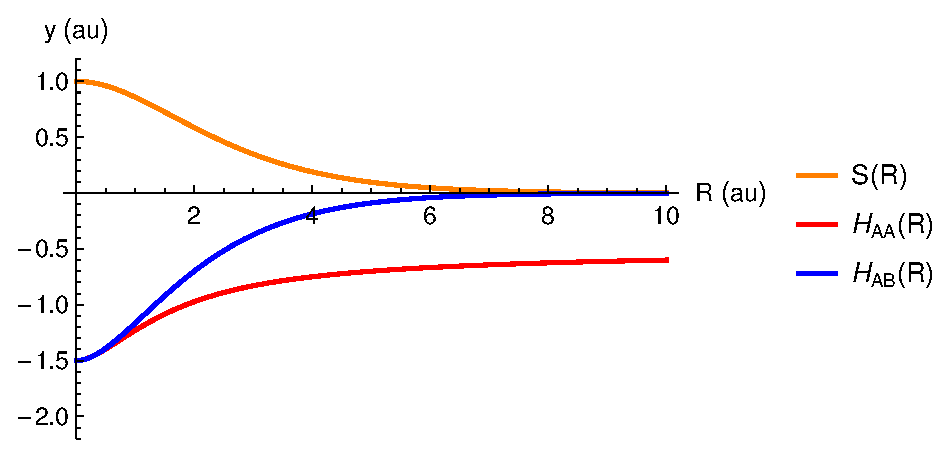
\includegraphics[scale=0.75]{h2_cation.eps}
  \caption{For $\gamma=1$, the overlap ($S(R)$),
    the diagonal element of the Hamiltonian ($H_{AA}$), and the off-diagonal
    element of the Hamiltonian ($H_{AB}$) is shown as a function of $R$.}
  \label{fig:mat_elem}
\end{figure}

{\color{blue}
  At $R\rightarrow \infty$, the overlap ($S(R)$) and the off-diagonal element of the
  Hamiltonian ($H_{AB}(R)$) both approach 0 indicating that the two H nuclei are completely
  separated and non-interaction. Meanwhile, the diagonal element of the Hamiltonian
  ($H_{AA}(R)$) approach -1/2 Hartree as $R\rightarrow\infty$. At $R\rightarrow 0$,
  the H atoms are at maximal overlap and the electronic bonding energy becomes more negative
  and finite.}
\\

\noindent c) Repeat previous question for $\epsilon_{\pm}(R)$, using your insight from
those answers. Then add the nuclear repulsion and plot both energy levels. Deduce the
bond length and well-depth $D_e$ for this approximate calculation.

\begin{figure}[H]
  \centering 
  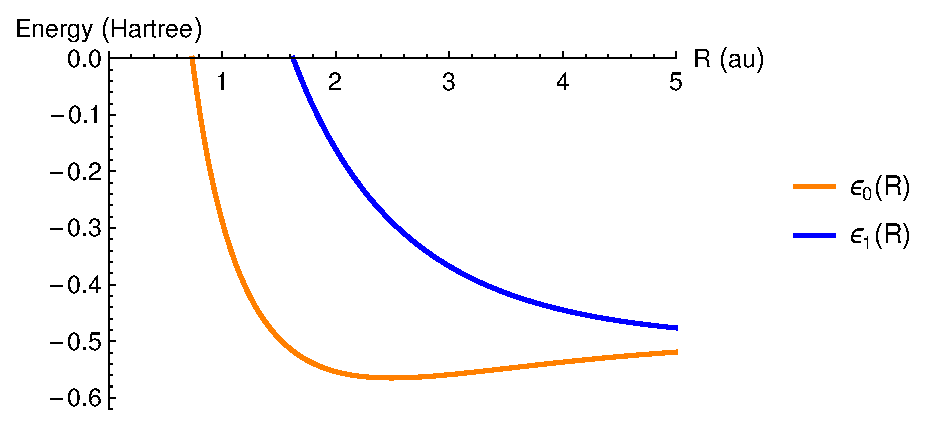
\includegraphics[scale=0.75]{h2_cat_curve.eps}
  \caption{The ground state curve ($\epsilon_1$) and first excited
    state curve ($\epsilon_1$) are shown as a function of
    the distance between two H nuclei ($R$).}
  \label{fig:cat_curve}
\end{figure}

{\color{blue}
  The well-depth $D_e$ is approximately 0.55 Hartree and the bond
  length is approximately 2.5 au.}
\\

\noindent d) Repeat $(b+c)$ using $\gamma = 1 + 1/2^R$, but only for the lower curve.
Plot all quantities on the same plots as before, and explain all differences. Calculate
bond length and depth. Compare with exact answers (google or NIST).

\begin{figure}[H]
    \centering
    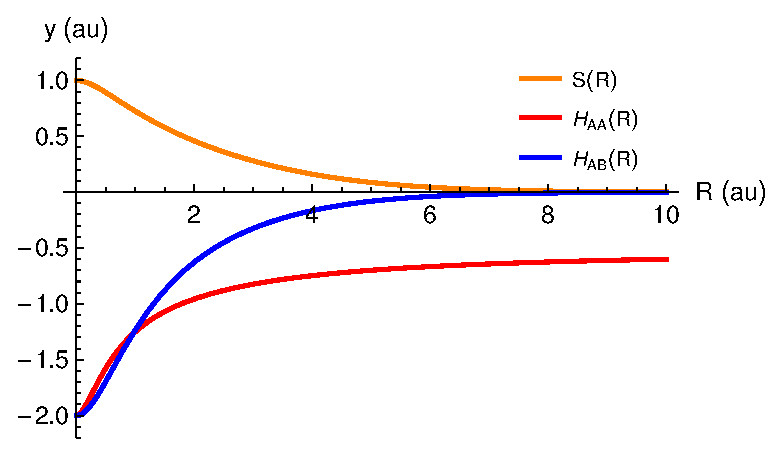
\includegraphics[width=0.495\textwidth]{h2_gamma.eps}
    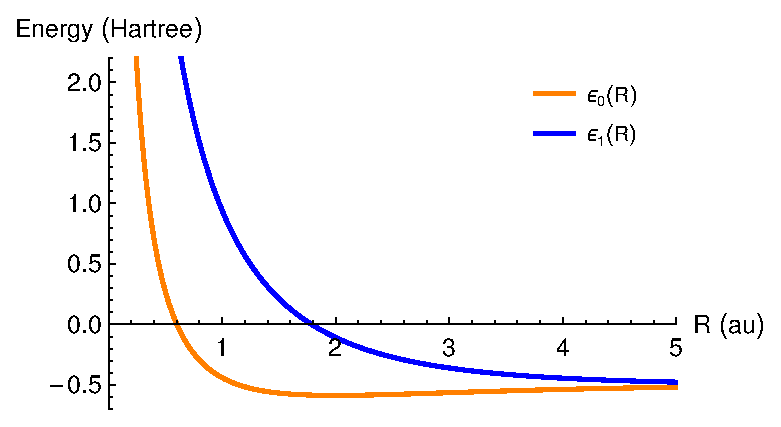
\includegraphics[width=0.495\textwidth]{h2_gamma_curve.eps}
    \caption{Side by side figures of the effect when $\gamma= 1 + 1/2^R$
      on the $S(R)$, $H_{AA}(R)$, $H_{AB}(R)$, and energy curve of H$_2^+$ (left).
      The ground state ($\epsilon_1$) and first excited state curves ($\epsilon_1$)
      are shown (right).}
    \label{fig:sidebyside}
\end{figure}

{\color{blue}
  Well-depth is approximately 0.1 Hartree and exact well-depth is 0.102 Hartree
  (google).
  Bond length is approximately 2.1 au and reported equilibrium bond length
  of H$_2^+$ is $2.0\pm0.1$ (DOI: 10.1063/1.1674078).
}

\pagebreak

\section*{H$_2$}

\noindent a) Plot the HF binding energy of H$_2$, approximating the Hartree energy
as $U_H=\frac{5\gamma}{8}(1+e^{-x/4})$, using the HF energy $E=2\epsilon + U_H/2$,
and using the same $\gamma$ as in H$_2^+$.

\begin{figure}[H]
  \centering
  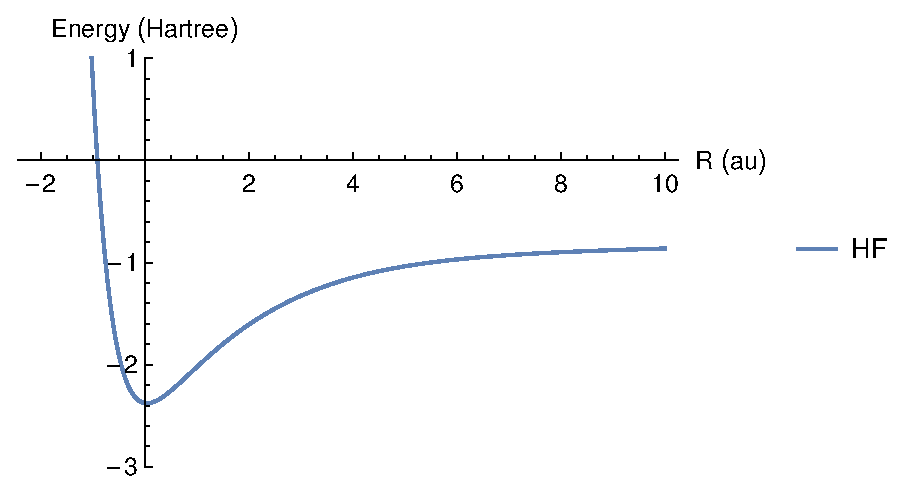
\includegraphics[scale=0.75]{hf_energy.eps}
  \caption{Apprxominated HF binding energy of H$_2$ for $\gamma=1$.}
\end{figure}

\noindent b) Find the equilibrium bond distance and well-depth from your curve.
Compare with the accurate HF values and comment.
\\

{\color{blue}
    The well-depth is approximately 1.15 Hartree and the equilibrium bond
    distance is approximately 1.22 au. Accurate HF values for equilibrium
bond distance and well-depth are 1.39 au and 1.13 Hartree, respectively.}
\\
  
\noindent c) Estimate the effective force constant and hence harmonic vibrational
frequency and compare with exact value. Comment on what this means about the error
in the shape of the curve
\\

{\color{blue}
  Computed effective force constant $\frac{d^2E_{\text{binding}}}{dR^2}\bigg|_{R=R_e}=0.804$
  au which is lower than the exact value 1.018 au.
}
\\

\noindent d) Plot the Morse potential corresponding to H$_2$ on the same plot. Plot
their difference near the equilibrium bond length. This would be the correlation
energy if both curves were accurate. The correlation energy at equilibrium is -0.042H.
Compare with the He atom. Comment on the variation of $E_C$ with $R$ and what this
means for HF errors in bond lengths.
\\

\begin{figure}[H]
  \centering
  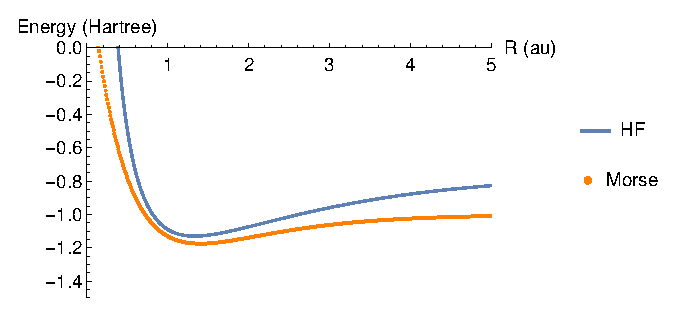
\includegraphics[scale=1]{hf_morse_comp.eps}
  \caption{Morse potential corresponding to H$_2$ and HF binding energy
  of H$_2$ are shown.}
\end{figure}

{\color{blue}
  $E_C$ is smaller near the equilibrium distance ($R_e$). Anything outside $R_e$
  then $E_C$ grows.
}

\begin{figure}[H]
  \centering
  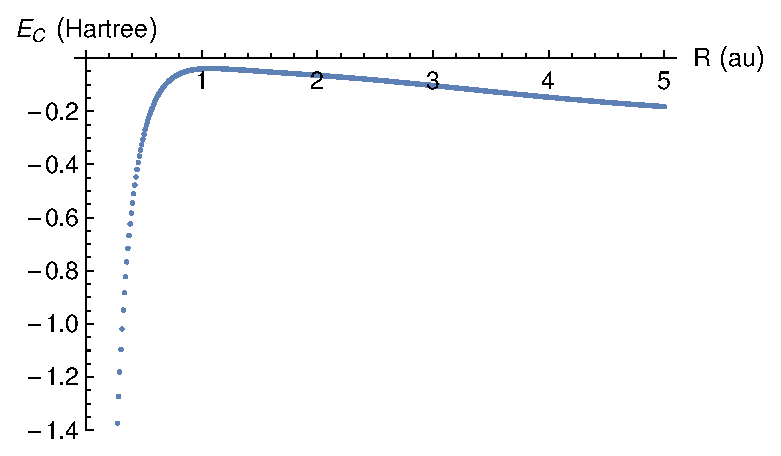
\includegraphics[scale=0.8]{diff_hfmorse.eps}
  \caption{Difference between the Morse potential and HF curve of H$_2$
    shown near the equilibrium bond length.}
\end{figure}

\noindent e) Consider your curve as $R\rightarrow\infty$. What value is it
approaching? Is this correct? If not, why not? What should differ in your energy
expression?
\\

{\color{blue}
  The binding energy for H$_2$ approaches -11/16 Hartrees or -0.6875 Hartrees.}

\pagebreak

\section*{Analyzing Experimental Numbers on Diatomic Isotopes}

This problem uses the first three rows of Table 7.2 of BRR.  Ignore the last two columns
($B$ and $\alpha_e$) which refer to rotations.  You will want to type the rest into
some software, such as excel.  Do all calculations in Hartree.
\\

\noindent a) Just by staring at the numbers, can you spot two (large) typos in the table? One has a
wrong digit, another has a misplaced decimal point. Correct them. Check the reduced mass
results and convert into atomic units.
\\

{\color{blue} Incorrect vibrational frequency for D$_2$ and equilibrium
  bond distance of H$_2$.
}
\\

\noindent b) Given the results for $v_e$, $x_e$ and $y_e$, calculate the zero-point
energy in each well.
\\
{\color{blue} $E_{\text{vib}}(\nu)=hv_e[(\nu+\frac{1}{2})-x_e(\nu+\frac{1}{2})^2+y_e(\nu+\frac{1}{2})^3]$
  for $\nu={0,1,...}$}
\begin{table}[H]
  \caption{Vibrational zero point energies (ZPE) in Hartrees}
  \centering
  \begin{tabular}{c|c}
    Molecule & ZPE \\
    \hline
    H$_2$ & 0.00989 \\
    HD    & 0.00858 \\
    D$_2$ & 0.00704
  \end{tabular}
\end{table}

\noindent c) Add your zero-point energies to each $D_0$ to estimate $D_e$. What should
you find, and do you find it?
\\
\begin{table}[H]
  \caption{Well-depth ($D_e$) in Hartrees}
  \centering
  \begin{tabular}{c|c}
    Molecule & $D_e$ \\
    \hline
    H$_2$ & 0.174424 \\
    HD    & 0.174423 \\
    D$_2$ & 0.174434
  \end{tabular}
\end{table}

{\color{blue} The estimated $D_e$ is close e.g. H$_2$ well-depth is 0.174486 Hartrees.}

\noindent d) Calculate the force constant for each well. What should you find,
and do you find it?

\begin{table}[H]
  \caption{Force constant $k$}
  \centering
  \begin{tabular}{c|c}
    Molecule & $D_e$ \\
    \hline
    H$_2$ & 1.0184 \\
    HD    & 1.0204 \\
    D$_2$ & 1.0237
  \end{tabular}
\end{table}

\noindent e) Using the spectroscopic formula for the energies, how many vibrational
levels do you expect each well to bind?
\\

{\color{blue} Estimating with the Morse potential, the H$_2$
  has 14 vibrational levels. This will be the same for the other
  isotopes.
}

\noindent f) Repeat (e) assuming each well was purely parabolic.
\\

{\color{blue} 8 vibrational states for the H$_2$.}
\\

\noindent g) For H$_2$ only, plot the harmonic levels and the true levels.
\\
\begin{figure}[H]
  \centering
  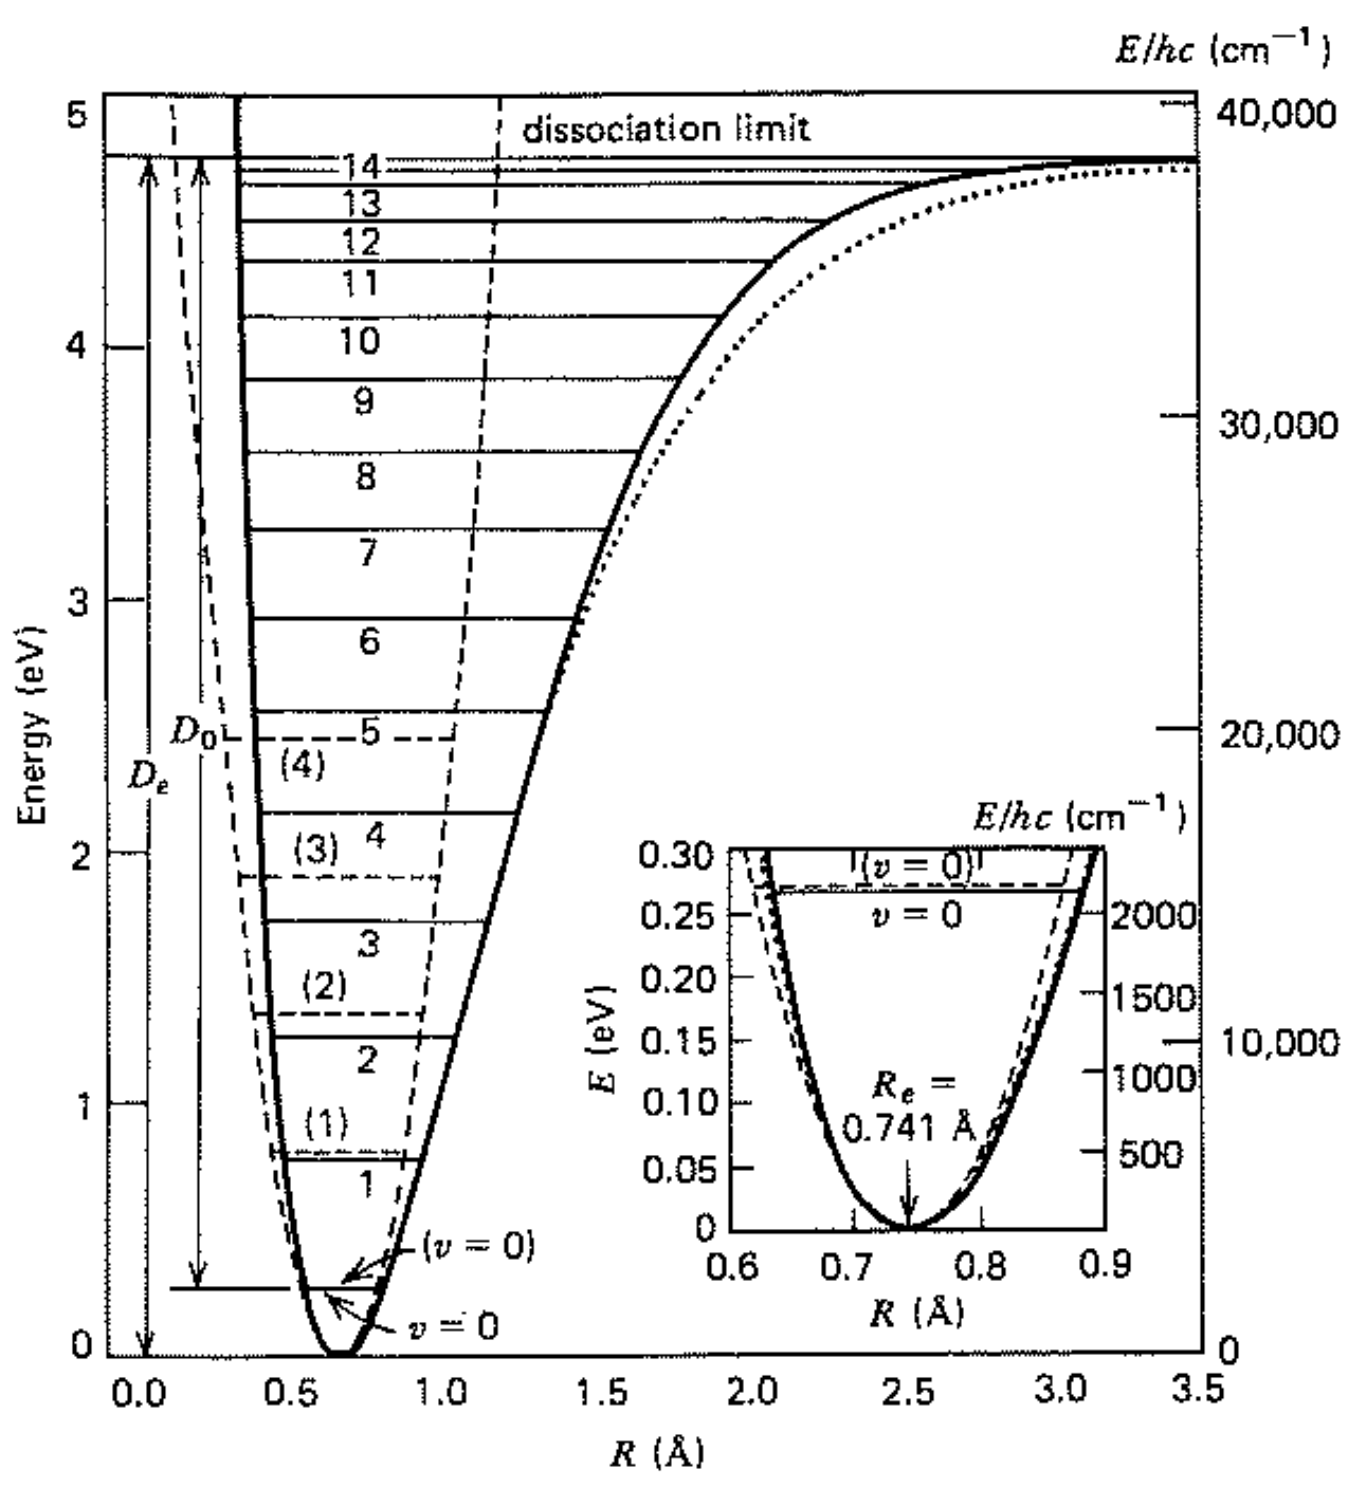
\includegraphics[scale=0.15]{harmonic_true.png}
\end{figure}

\noindent h) Make the row of numbers for T$_2$.
\begin{table}[H]
  \caption{Vibrational constants for T$_2$}
  \centering
  \begin{tabular}{c|cc}
    Molecule &$\mu$ (amu) & $R_e$ (Angstrom)\\
    \hline
    T$_2$ & 1.5 & 0.7412 \\
  \end{tabular}
\end{table}

\pagebreak

\section*{Theoretical Approach to Diatomic Vibrations}

The energy levels of a Morse potential $V_0(\exp(-2\alpha (R-R_0)) -2 \exp(-\alpha (R-R_0)))$
are
\begin{equation}
\epsilon_n = -V_0\, \left( 1 - \frac{\alpha (n+\frac{1}{2})}{\sqrt{2\, \mu\, V_0}} \right)^2
\end{equation}
where $n$ takes all integer values from 0 up to where the term in brackets
becomes negative, and $\mu$ is the mass.
\\

\noindent a) Find the minimum position and well-depth, and so relate $V_0$ and $R_0$ to
quantities in molecular binding curves (if they had this shape).
\\

{\color{blue} Let $R'=R-R_0$ and find the minimum of Morse potential
  \begin{align}
    \frac{dV(R')}{dR'} = -2\alpha V_0(e^{-2\alpha R'}-e^{-\alpha R'}) = 0.
  \end{align}
  Since the minimum of the Morse potential is 0 at $R'=R-R_0=0$, then $V_0=D_e$ implying
  $R_0=R_e$.
}
\\

\noindent b) Expand the Morse potential around its minimum, and so find a formula for $\alpha$
in terms of the harmonic approximation to a molecular well.
{\color{blue}
\begin{align*}
  V(R) & = V_0(e^{-2\alpha(R-R_0)}-2e^{-\alpha(R-R_0)}) \\
  & = D_e(e^{-2\alpha(R')}-2e^{-\alpha(R')}) \\
  & = D_e(1-2\alpha R' + 2\alpha^2R'^2 -2(1-\alpha R' +\frac{1}{2}\alpha^2R'^2) \\
  & = -D_e + D_e\alpha^2R'^2 \\
  k & = \alpha^2D_e \\
  \alpha & = \sqrt{k/D_e}
\end{align*}
}

\noindent c) Deduce expressions for $x_e$ and $y_e$ for this well, in terms of the molecular
properties.
{\color{blue}
  \begin{align*}
    \epsilon_n & = -D_0\, \left( 1 - \frac{\alpha (n+\frac{1}{2})}{\sqrt{2\, \mu\, D_e}} \right)^2 \\
    & = - D_e(1 - \sqrt{\frac{2}{\mu D_e}}\alpha(n+\frac{1}{2}) +\frac{\alpha^2}{2\mu D_e}(n+\frac{1}{2})^2)\\
    & = - D_e + \omega(n+\frac{1}{2})(1-x_e(n+\frac{1}{2})+y_e(n+\frac{1}{2})^2) \\
    y_e & = 0 \\
    \omega & = \sqrt{\frac{2 D_e}{\mu}}\alpha \\
    \omega x_e & = \frac{\alpha^2}{2\mu} \\
    x_e & = \frac{\alpha}{\sqrt{8\mu D_e}}
  \end{align*}
  }

\noindent d) From your expression for $x_e$, find a combination of $D$, $x_e$, and $\nu_e$
that should be mass independent, and use the data to check if it is.  Compare with
Morse result and comment.
\\

\pagebreak
\noindent e) How many levels does your Morse potential predict for H$_2$?  Compare with the
perturbative answer and the harmonic approximation and comment.

{\color{blue}
  \begin{align*}
    \epsilon_e & = -D_e[1-\frac{\omega}{2D_e}(x+\frac{1}{2})]^2 \\
    n_{\text{max}} & = \frac{2D_e}{\omega} - \frac{1}{2} = \frac{x_e^{-1}-1}{2} = 16\times9
  \end{align*}
  
  Morse predicts 16 levels and harmonic approximation predicts 8. The reality is 14.}
\\

\noindent f) Add the Morse levels to your plot of H$_2$ levels, and compare with true levels.
\\

{\color{blue} Morse potential will be close but, not perfect at higher levels.}

\pagebreak

\section*{General Problems about Diatomics from BRR}

  1. \textit{Ionic bonds:} Use Table 7.3 to deduce the values of B and $\rho$ used in
  Eq (7.43). Are they reasonable? How might you have found them without reverse engineering?
  Is the agreement between calculation and experiment accurate enough by quantum chemistry
  standards? Identify which components of a KS calculation are being approximated by the
  separate terms in Eq (7.44).

  {\color{blue}
  \begin{align}
    V_{\text{rep}}(R) & = Be^{-R/\rho} \label{eqn:born_mayer}\\
    E(R) & = -\frac{q_1q_2}{4\pi\epsilon_0R} + V_{\text{rep}}(R)
    \label{eqn:dissociation}
  \end{align}

  $E(R)$ is the ``ionic dissociation energy'' taken from BRR and $V_{\text{rep}}(R)$ is
  the Eq (7.43) or the Born--Mayer potential. With Table 7.3, we can reverse engineer
  from calculated $D_e$ to fit the exponential. The constants $B$ and $\rho$ are
  determined 33.056 and 2.324, respectively.

  \begin{figure}[H]
    \centering
    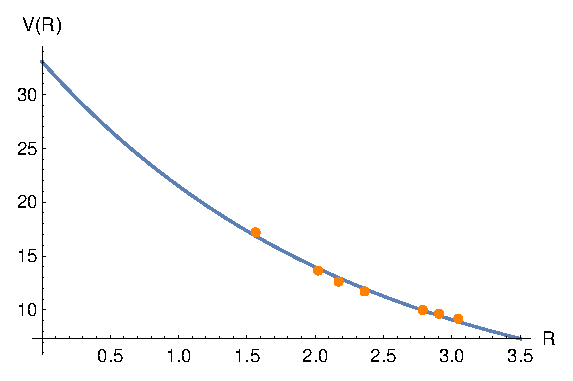
\includegraphics[scale=1]{fitted_rhoB.eps}
    \caption{Exponential fit for the Born--Mayer potential to determine $B$ and
      $\rho$ from Eqn. \eqref{eqn:born_mayer}.}
    \label{fig:fit}
  \end{figure}
  
  \begin{table}[H]
    \centering
    \caption{Ionic Bond Model and absolute difference between experiment and calculated
      in eV.}
    \begin{tabular}{cccc}
      Molecule & Calc. & Obs. & Diff \\
      \hline
      LiF  & 7.9996 & 7.983 & 0.017 \\
      LiCl & 6.513  & 6.648 & 0.135 \\
      NaCl & 5.616  & 5.750 & 0.134 \\
      KF   & 5.993  & 6.036 & 0.043 \\
      KI   & 4.458  & 4.601 & 0.143 \\
      RbCl & 4.835  & 4.917 & 0.082 \\
      CsCl & 4.692  & 4.870 & 0.178
    \end{tabular}
  \end{table}
  
  The error can be up to $\sim 0.2$ eV, or $\sim 3$ kcal/mol. It is fairly good for smaller
  ions within chemical accuracy of $\sim 1$ kcal/mol. However, the model does not do ``well''
  for large ions where errors can reach up to $\sim 3$ kcal/mol based on quantum chemistry
  standards.}
  \\
  \\
  \noindent2. \textit{Homonuclear diatomics:} Use Fig 7.14 to identify the error in a configuration
  in Table 7.5. Explain the labeling of the excited states in Table 7.6.
  \\

  {\color{blue}
  According to Fig 7.14, the molecular orbital configuration of N$_2$ is incorrect and it
  should be:

  N$_2$: KK$(2\sigma_g)^2(2\sigma_u)^2(3\sigma_g)^2(1\pi_u)^4$}
  \\

  {\color{blue}
  Molecular term symbols are defined
  \begin{equation*}
    ^{2S+1}|\Lambda|_{(g/u)}^{(+/-)}
  \end{equation*}
  \noindent where $S$ is the total spin angular momentum, $\Lambda$ is the total orbital
  angular momentum, $g/u$ corrpondes to symmetry of the electronic wavefunction with repect
  to inversion through this center, and $+/-$ applies only to $\Sigma$ states labeling
  symmetry of the wavefunction with respect to the reflection in a plane containing the
  nuclei.}
  \\
  \\
  \noindent3. \textit{Electronegativity:} Read 7.7 and explain the spelling error in FONClBrISCHP.
  \\

  {\color{blue}
  Based on the Pauling scale, FONClBrISCHP has the incorrect order from most to least electronegative
  atoms. The correct order is FOClNBrISCHP.}
  \\
  
  \noindent4. \textit{Potential energy surfaces:} Read 7.8 and explain the Massey criterion.
  When can curves cross and when do they not? If curves do not cross, can molecules change
  PES?
  \\
  
  {\color{blue}
  The Massey adiabatic criterion is the transition period ($\Delta t$) at which the molecule
  on one potential energy surface (PES) encounters another PES within $\Delta E$ over a range
  $\Delta R$. Yes, the molecule can change PES if the curves do not cross e.g. phosphorescence.}
  \\
  \\
  \noindent5. \textit{Hydrides and isoelectronic series:} Read 7.9 and explain what is special
  about diatomic hydrides. Explain how hydrogen bonding upsets trends in boiling point
  data. Do problem 7.20.
  \\
  
  {\color{blue}
  Nearly all diatomic hydrides in the first row are highly reative species that are
  observed mainly in high-temperature systems. Certain trends follow such as strength
  of bonding indicated by increasing $D_e$, shortening bond distances $R_e$, and
  increasing vibrational frequency $\tilde{v}_e$ from LiH to HF. Typo on pg 220, the
  boiling trends where H$_2$O boiling point is written 0.0$^{\circ}$C but, H$_2$O boils
  at 100$^{\circ}$C. Hydrogen bonding}
  \\
  
  Problem 7.20) Predict dissociation energy, equilibrium internuclear distance $R_e$,
  and vibration frequency $\tilde{v}_e$ by extrapolation from the data in Table 7.9.
  \\

  \color{blue}
  Extrapolated results with linear regression between the observable and molar mass.
  \\
  
  a) At$_2$: $\tilde{v}_e=22$ cm$^{-1}$, $R_e=3.349$ angstroms, $D_0=0.79$ eV.

  b) DAt: $\tilde{v}_e=1705$ cm$^{-1}$, $R_e=1.954$ angstroms, $D_0=1.81$ eV.

  c) Fr$_2$: $\tilde{v}_e=12.72$ cm$^{-1}$, $R_e=5.302$ anstroms, $D_0=0.41$ eV.
\end{document}
